\documentclass[letterpaper, 10 pt, conference]{ieeeconf}
% Comment this line out if you need a4paper

%\documentclass[a4paper, 10pt, conference]{ieeeconf}
% Use this line for a4 paper

\IEEEoverridecommandlockouts
% This command is only needed if
% you want to use the \thanks command

\overrideIEEEmargins
% Needed to meet printer requirements.

% See the \addtolength command later in the file to balance the column lengths on the last page of the document

\usepackage{graphics} 	% for pdf, bitmapped graphics files
\usepackage{graphicx}
\usepackage{epstopdf}
\usepackage{epsfig} 	% for postscript graphics files
\usepackage{times} 		% assumes new font selection scheme installed
\usepackage{balance}
\usepackage{color}
\usepackage[utf8]{inputenc}
\usepackage{amsmath}
\usepackage{booktabs}
\usepackage{amssymb}
\usepackage{theorem}
\usepackage{algorithm}
\usepackage{algorithmic}
\usepackage{tabularx}
\usepackage{indentfirst}
\usepackage{subcaption}


\newtheorem{proposition}{Proposition}
\newtheorem{theorem}{Theorem}
\newtheorem{corollary}{Corollary}
\newtheorem{remark}{Remark}
\newtheorem{lemma}{Lemma}
\newtheorem{assumption}{Assumption}
\newtheorem{definition}{Definition}
\newcommand{\BH}[1]{\textcolor{red}{#1}}

\newcommand{\Proof}{\noindent \textit{Proof.}$\;\;$}

\title{\bf Tree Structured Traffic Coordination with Decentralized Optimization}

\author{Xiaotian Fang, Yuning Jiang}

\begin{document}
\maketitle
\thispagestyle{empty}
\pagestyle{empty}

\begin{abstract}
	This paper proposes a distributed model predictive control algorithm for tree structed traffic coordination problem by using two dimensional models for autonomous vehicles. With the defination of conflict zone, A complete strategy is proposed to model the structe of the vehicles' network to a tree topology. The shape of vehicles is also be considered in this paper, and the collision avoidance constraints are formulated by enclosing each vehicle in an ellipse. Then the closed-loop control scheme is constrcuted based on a model predictive method. And a decentralized optimization method over tree graph, called multi-sweep method, is used to solve the traffic coordination problem in each MPC loop. Two numerical cases under two realistic senerios are introduced to illustrate the performance of the proposed method.
\end{abstract}


\section{Introduction}
Autonomous vehicles have received much attention in recent years. Interest in coordinating vehicles such as unmanned ground vehicles (UGVs)~\cite{Hult2015}, unmanned underwater vehicles (UUVs)~\cite{Yan2018}, and unmanned air vehicles (UAVs)~\cite{Keviczky2008} has been on the rise in control system community. Many methods~\cite{Kowshik2011,Lee2012,Campos2013,Chen2016} for coordinating self-driving cars at traffic intersections have been proposed in the past few years. For example, in~\cite{Chen2016}, a cooperative management system has been proposed to coordinate cars at traffic intersections. A connected communication network has been designed for coordination of vehicles in~\cite{Lee2012}. Moreover, a receding horizon based the cooperative approach has been developed in~\cite{Campos2014}.

The coordination of autonomous vehicles can be formulated as a structured optimal control problem. Concerning various scenarios, different methods has been proposed to model collision avoidance constraints. Based on double integrator dynamics, a spatial method has been proposed in~\cite{Katriniok2017}, which enforces a safety distance between two vehicles. Moreover, in~\cite{Hult2015} a collision avoidance controller has been developed, which allows only one car on the intersection at a time. In~\cite{Hafner2013}, hybrid system theory has been used to address the traffic control problem under a verifiable safety condition.

MPC controllers for traffic coordination have been developed in~\cite{Campos2013,Campos2014}. Due to the fast dynamic of autonomous vehicles, a real time iteration based strategy was designed in~\cite{Frasch2013} for obstacle avoidance constraints. If we consider the connection structure of vehicles as a mutli-agent network, if a vehicle is plugged or unplugged from the network, this results in a change of the number of total differential states in the optimal control problem. In~\cite{Shi2018}, a closed-loop control scheme with recursive feasibility guarantee for time-varying networks has been proposed. 

Modern wireless networks can provide a reliable and fast channel for information exchange between multiple agents. Many researchers have proposed methods that exploit the network structure of interconnected vehicles to solve multi-vehicle coordination problem in a distributed manner. By distributing the sensitivity evaluation in sequential quadratic programming (SQP)~\cite{Nocedal2006}, a primal decomposition based SQP method~\cite{Hult2016} was proposed to solve the optimal control problem. The follow-up asynchronous version~\cite{Zanon2017} reduces the communication overhead. While this method is distributed, the corresponding QP is solved by one car, which is chosen as the central unit. A fully parallalizable MPC based approach was proposed in~\cite{Katriniok2017}. Another class of distributed optimization methods are based on the alternating direction method of multipliers (ADMM)~\cite{Boyd2011}. In~\cite{Wang2015}, ADMM has been illustrated to be applicable for noncovex optimization problem. An ADMM based nonlinear MPC approach proposed in~\cite{Ferranti2018} aims to coordinating multiple vessels at intersections. Moreover, in~\cite{Jiang2017} ALADIN has been used to solve the traffic optimal control problem in a distributed way by negotiating a time schedule between the vehicles. 

Meanwhile, a huge amout of research focus on distributed optimization algorithms over networks with tree topology, which arise in many applications such as traditional optimal control problems~\cite{Bellman1966} or receding horizon control problems~\cite{Ljung1999}, where linear trees occur, scenario multi-stage MPC problems~\cite{Bernardini2011,Kouzoupis2018,Lucia2014}, which have less trivial tree structures, or radial power grid networks that possess non-trivial tree structure too~\cite{Kekatos2012,Peng2014}.

This paper is mainly based on the work of ~\cite{Jiang2017,Shi2018} for coordination of vehicles at traffic intersections, and ~\cite{JiangTree} for decentralized optimization method over tree graphs. Modeling the vehicles in two dimensions to enclose each vehicle by a two-dimensional ellipsoid and to enforce a minimal sfety distance between them for collision avoidance. Conflict region and complete regulations are defined to help model the connections between vehicles to tree topology. The closed-loop scheme is constructed by model predictive control method while the resulting online optimization problem with tree topology is solved with multi-sweep method. 

The rest of this paper is organized as follows. Section~\ref{sec::model} presents the model of the vehicle and the frame of local and global coordinates. Section~\ref{sec::cons} introduces a tractable formulation of the collision avoidance constraint. Section~\ref{sec::form} summarizes the optimal control problem and its reformulation to tree-topology problem, and meanwhile briefly introduces the solving approach, multi-sweep method. Section~\ref{sec::mpc} presentsthe closed-loop MPC implemention details. Two realistic case studies are presented in Section~\ref{sec::case}. At last, Section~\ref{sec::conc} concludes this paper.

\section{System Model}
\label{sec::model}
In this paper, we consider a traffic system with some vehicles under several realistic scenarios. In order to formulate the coordination problem, we have following Assumptions:
\begin{itemize}
	\item[\textbf{A1}] The vehicles follow fixed, predetermined paths.
	\item[\textbf{A2}] Vehicle states are measurable without uncertainty.
	\item[\textbf{A3}] Vehicles in differnet paths only need to consider each other inside the conflict regions.
	\item[\textbf{A4}] Vehicle paths are straight outside the intersection.
	\item[\textbf{A5}] All vehicles are equipped with V2V communication devices.
	\item[\textbf{A6}] The MPC solutions at time $k$ are available to all vehicles at time $k+1$.
\end{itemize}


\subsection{Vehicle Kinematics}
Let $N_v$ denote the number of vehicles and $\mathcal{V} := \{1,\dots,N_v\}$. According to assumption A1, the position of vehicle $i$, which moves along a fixed path, can be parametrized by only one scalar $s_i$. Let $x_{i,k} = [s_{i,k};v_{i,k}]$ denote the state of each vehicle $i\in \mathcal{V}$ at time $ k\in \mathbb{Z}_0^{K} = \lbrace t_0,t_1,\dots,t_K \rbrace$, where $s_{i,k}$ and $v_{i,k}$ respectively represent the scalar longitudinal position and velocity. And control varaible $u_{i,k}$ represents the saclar longtitudinal acceleration. Then, each vehicle is modeled as a discrete time double integartor
\begin{equation}
x_{i,k+1} = A\cdot x_{i,k} + B\cdot u_{i,k}\;,
\end{equation}
where $A=[1,h;0,1]$, $B=[0;h^2/2]$, and $h$ denotes one time interval.

Meanwhile, considering the traffic regulations and the parameters of real vehicles. Each vehicle is supposed to follow the state and control constraints below:
\begin{align}
v_i^{min} \leq v_{i,k} \leq v_i^{max} \; , \label{eq::statecon} \\
u_i^{min} \leq u_{i,k} \leq u_i^{max} \; , \label{eq::contcon}
\end{align}
In the following, we use shorthand
$
h(x_{i},u_{i})\leq 0
$
to collect~\eqref{eq::statecon} and~\eqref{eq::contcon} for all $k\in \mathbb{Z}_0^{K}$.

\subsection{Local and Global Coordinate Frames}
The position of vehicles in 2-D can be given by function $p_i:\mathbb{R}\rightarrow \mathbb{R}^2$,
\[
p_i(s_{i,k}) =(p_{i,x}(s_{i,k}),p_{i,y}(s_{i,k}))\;.
\] 
For the given predetermined path, refer to~\cite{Katriniok2019}, we use $n_p$-th order B-splines to represent it,
\begin{align}
\left[
\begin{matrix}
p_{i,x}(s_{i,k}) \\[0.16cm]
p_{i,y}(s_{i,k})
\end{matrix}
\right] =
\left[
\begin{matrix}
\sum_{l=0}^{n_{p}}\alpha^{x,l}B^{x,l}_n(s_{i,k}) \\[0.16cm]
\sum_{l=0}^{n_{p}}\alpha^{y,l}B^{y,l}_n(s_{i,k})
\end{matrix}
\right]\;.
\end{align}
Similarly, the navigation angle $\theta(s_{i,k})$ can be also represented as functions of $s_{i,k}$. In the following, we use notation $p_{i,k}:=p(s_{i,k})$ and $\theta_{i,k}:=\theta(s_{i,k})$.

\subsection{Vehicle Shape}
\begin{figure}[htbp!]
	\centering
	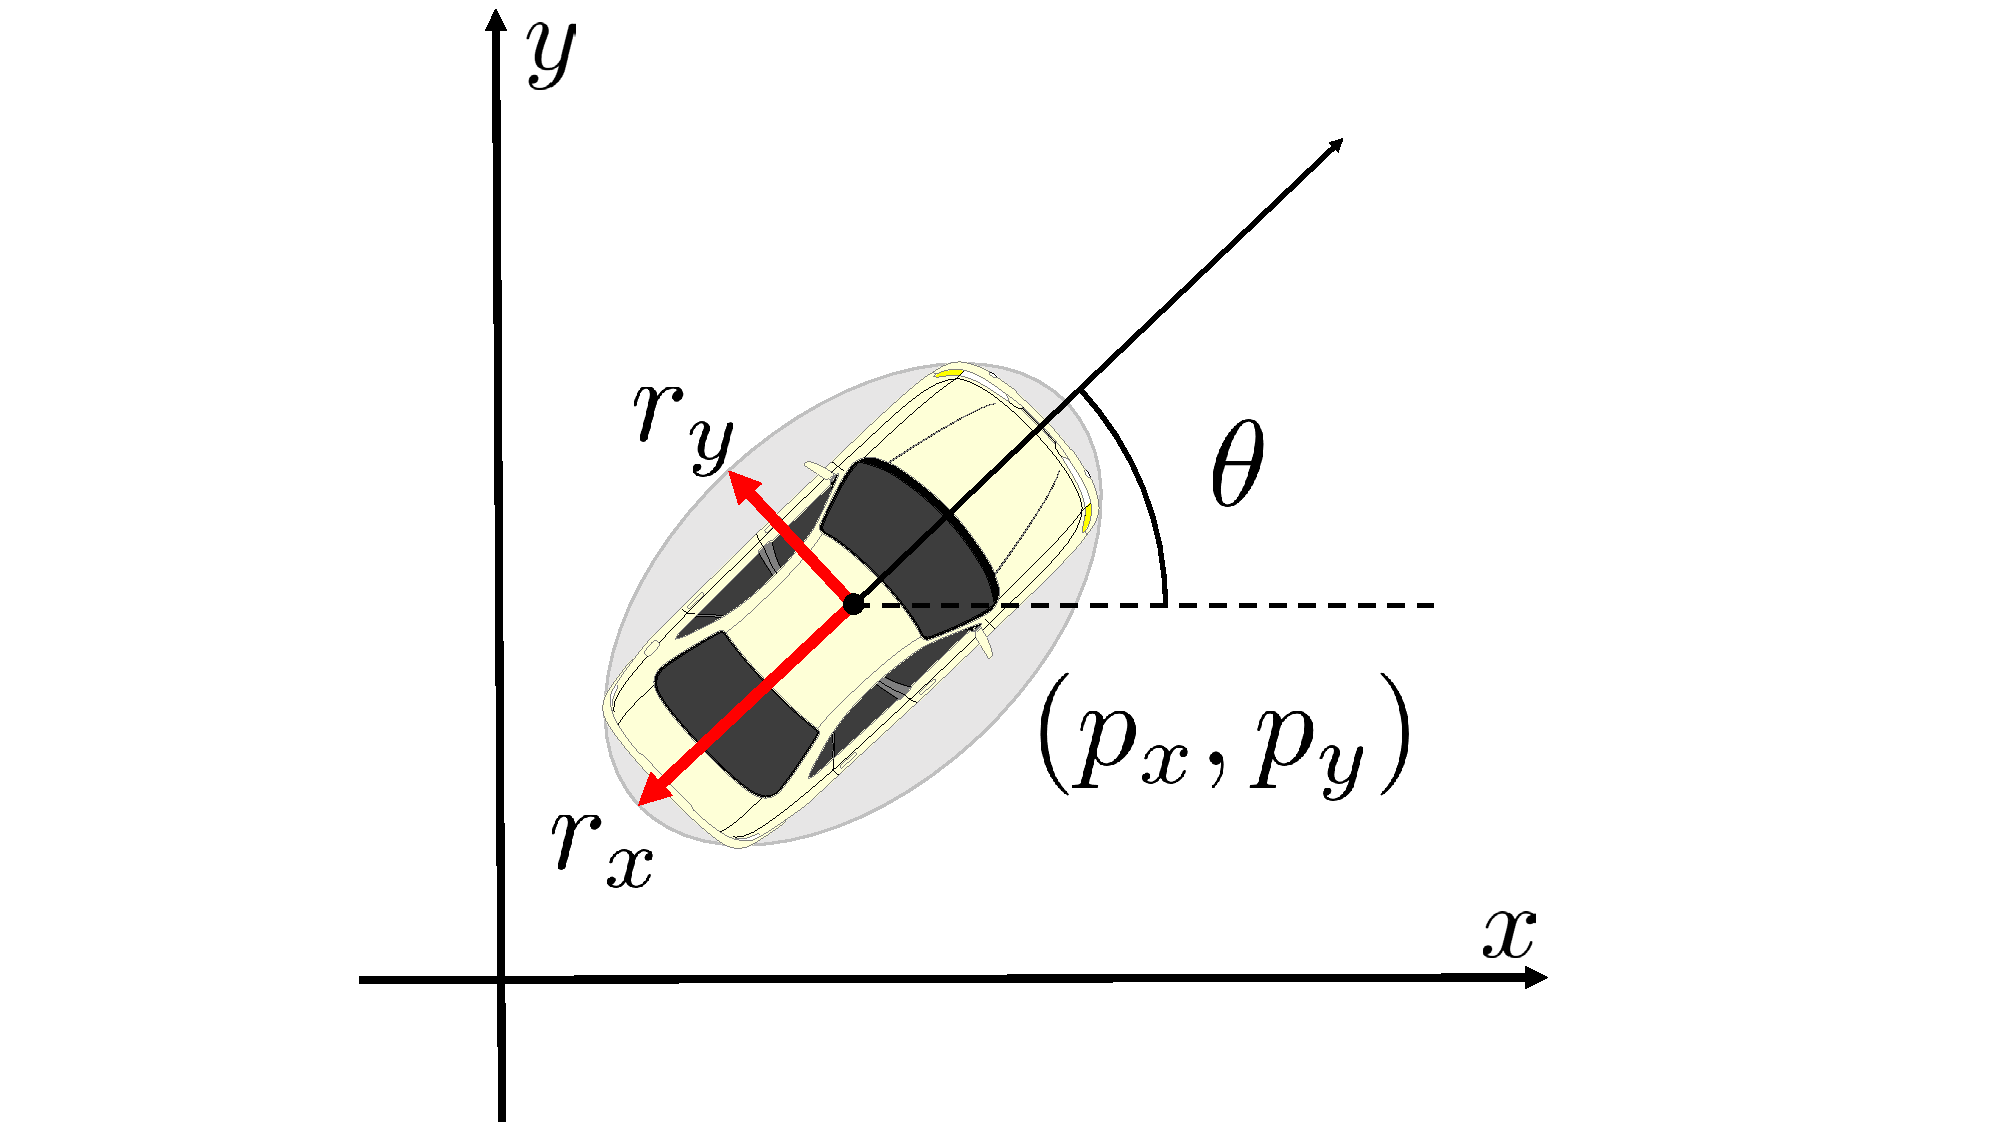
\includegraphics[width = 0.8\linewidth]{pic/car}
	\caption{Elliptical vehicle model.}
	\label{fig::car}
\end{figure}
In order to analyze the distance between two vehicle in 2-D plane, we model vehicle as an ellipse as shown in Figure~\ref{fig::car}.
We denote the shape ellipse by $\mathcal{E}(p_{i,k},\mathcal{Q}(\theta_{i,k}))$
with center $p_{i,k}$ and shape matrix
\begin{equation}\notag
\mathcal{Q}(\theta_{i,k})=
\begin{bmatrix}
r_{x}^2\cos^2 \theta_{i,k}+r_{y}^2\sin^2 \theta_{i,k} , \;
0.5\sin 2\theta_{i,k}(r_{x}^2-r_{y}^2) \\[0.16cm]
0.5\sin 2\theta_{i,k}(r_{x}^2-r_{y}^2) ,\;
r_{x}^2\sin^2 \theta_{i,k}+r_{y}^2\cos^2 \theta_{i,k}
\end{bmatrix}.
\end{equation}
Here, both the center of the ellipse and the shape matrix are parameterized over $s_{i,k}$. And $(r_{x}, r_{y})$ denotes the length of semi-major radius of ellipses.


\section{Collision Avoidance}
\label{sec::cons}
\subsection{Conflict Region}
For vehicle $i$, we define the conflict region 
\[
\mathcal{C}_i:=[s_i^{in},s_i^{out}]\;,
\]
 Where $s_i^{in}$ and $s_i^{out}$ denote the path coordinates of conflict region's entry and exit, respectively. Before vehicles enter the conflict region, let assumption A3 hold, vehicles in differnt paths move independently such that we only need consider rear-end collision. Once vehicles has been inside the intersection, the possibility of side collision between vehicles in different lanes occurs. Notice that the choosing principles of conflict region might have some difference in different scenerios, we need to analyse specific scenerios to acquire a suitable conflict region. Some articles could be refered here~\cite{Hult2019}~\cite{Katriniok2019}. And in the case study section, we will define conflict region specificly in two different scenerios.

\subsection{Rear-end Collision Avoidance}
According to the assumption A3, we only need to consider the rear-end collision outside conflict region. Therefore, we denote by $a_i$ the vehicle which is ahead of vehicle $i$ in same path. When $s_{i,k}\notin\mathcal{C}_i$, vehicle $i$ only need to avoid rear-end collision with vehicle $a_i$. Since the path is straight before the intersection, as assumed in A4, the distance between two vehicles can be calculated by
\[
\delta_{i,a_i,k}=s_{i,k} - s_{a_i,k} - r_{i,x}-r_{a_i,x}\;.
\]
and the collision avoidance constraints can be given by
\begin{equation}
\label{eq::outcons}
\delta_{i,a_i,k} \leq \varepsilon_{out} \;,
\end{equation}
where $\varepsilon_{out}>0$ is the safe distance for vehicles outside conflict region.

\subsection{Side Collision Avoidance}
\begin{figure}[htbp!]
	\centering
	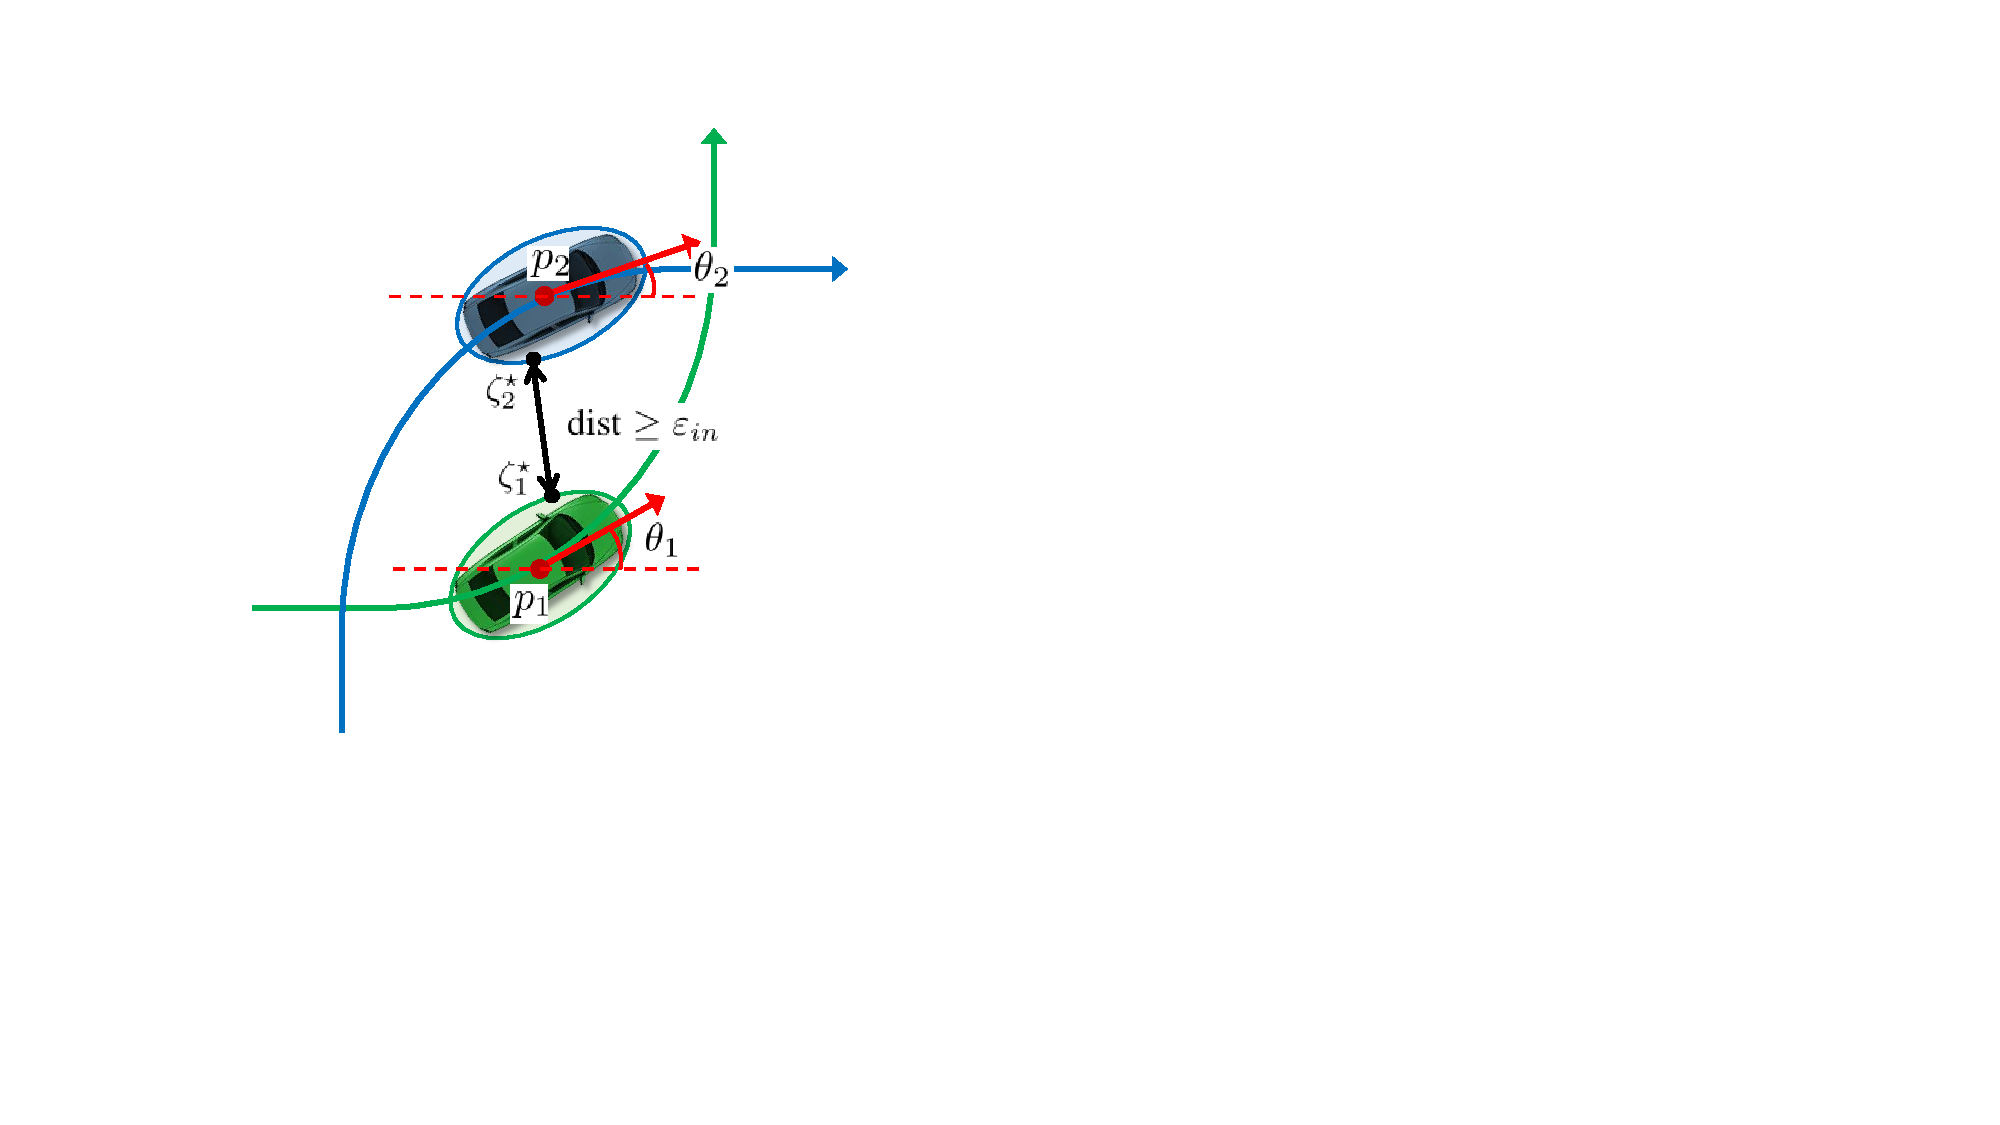
\includegraphics[width = 0.8\linewidth]{pic/ellipses}
	\caption{collision avoidance inside conflict region}
	\label{fig::ellipses}
\end{figure}
According to the defination of conflict region, vehicles start to consider the side collision when they enter the conflict region. In this phase, not only the rear-end collision at the same path but also the side collision between different lanes need to be considered. Here, we denote by $\mathcal{V}_i^\mathrm{b}$ the set of vehicles, except vehicle $i$, inside conflict region. Therefore, in order to avoid collision inside conflict region, we can enforce a safe distance between two vehicle ellipses inside the conflict region as shown in Figure~\ref{fig::ellipses}. For vehicle $i$, the collision avoidance constraint can be then formulated as
\begin{equation}
\label{eq::collision}
\text{dist}(\mathcal{E}(p_{i,k},\mathcal{Q}_i(\theta_{i,k})),\mathcal{E}(p_{j,k},\mathcal{Q}_j(\theta_{j,k})))\geq \varepsilon_{in}
\end{equation}
for all $j\in\mathcal{V}^\mathrm{b}_{i}$. Here, $\varepsilon_{in}$ denote the safety distance between vehicles inside the conflict region. However, constraint~\eqref{eq::collision} is not applicable in numerical algorithm design such that we introduce the following technical result.
\begin{theorem}
	\label{the::ColAvoid}	
	For any given two ellipsoids $\mathcal{E}(q_1,Q_1)$ and $\mathcal{E}(q_2,Q_2)$ in two dimensions, the inequality
	\[
	\text{dist}(\mathcal{E}(q_1,Q_1),\mathcal{E}(q_2,Q_2)) \geq d_{12}
	\]
	holds for a given distance $d_{12}$ if and only if there exist a
	$\delta = (\delta_1, \delta_2)\in\mathbb{R}^{2}$ such that
	\begin{equation}
	\label{eq::constraint_trans}
	\left\{
	\begin{array}{l}
	\|\zeta_1(\delta) - \zeta_2(\delta)\|_2\geq d_\mathrm{12}\;,\\[0.16cm]
	(\zeta_1(\delta)-q_{1})^\top Q_1^{-1} (\zeta_1(\delta)-q_{1})=1\;,\\[0.16cm]
	(\zeta_2(\delta)-q_{2})^\top Q_2^{-1} (\zeta_2(\delta)-q_{2})=1\;,\\[0.16cm]
	\delta \geq 0\;,
	\end{array}
	\right.
	\end{equation}
	where the functions $\zeta_1(\cdot)$ and $\zeta_2(\cdot)$ are given by
	\begin{equation}
	\label{eq::opt2}
	\begin{array}{rl}
	\zeta_1(\delta)\;=&[(I + \delta_2 Q_2^{-1}(I + \delta_1 Q_1^{-1}) - I]^{-1}\\[0.1cm]
	&[\delta_1(I + \delta_2 Q^{-1}_2)Q_1^{-1}q_{1}+\delta_2Q_2^{-1}q_{2}]\;,\\[0.2cm]
	\zeta_2(\delta)\;=&[(I + \delta_1 Q_1^{-1})(I + \delta_2 Q_2^{-1}) - I]^{-1}\\[0.1cm]
	&[\delta_2(I + \delta_1 Q_1^{-1})Q_2^{-1}q_{2}+\delta_1Q_1^{-1}q_{1}]\\[0.1cm]
	&\forall \delta\geq 0.
	\end{array}
	\end{equation}
\end{theorem}
\textit{Proof.}$\;\;$ The square of distance between two ellipsoids is given by the optimal value of the following optimization problem
\begin{align}
\label{eq::dist}
\min_{\xi_1,\xi_2} &\;\quad  \|\xi_1 - \xi_2\|_2^2\\\notag
\text{s.t.}\;&\quad \left\{
\begin{array}{ll}
1\;\geq\; (\xi_1-q_{1})^\top Q_1^{-1} (\xi_1-q_{1})&\mid \kappa_1\\[0.1cm]
1\;\geq\; (\xi_2-q_{2})^\top Q_2^{-1} (\xi_2-q_{2})&\mid \kappa_2
\end{array}
\right.\;.
\end{align}
We denote the Lagrangian of~\eqref{eq::dist} by
\[
\begin{split}
L(\xi,\kappa) =\;&\|\xi_1-\xi_2\|_2^2 +\kappa_1(\xi_1-q_{1})^\top Q_1^{-1} (\xi_1-q_{1}) \\[0.1cm]
& -\kappa_1+ \kappa_2(\xi_2-q_{2})^\top Q_2^{-1} (\xi_2-q_{2,k})-\kappa_2\;.
\end{split}
\]
Since~\eqref{eq::dist} is a strongly convex QCQP problem, whose feasible set has a non-empty interior, there is no duality gap. By expanding the first order optimality condition of~\eqref{eq::dist}, we find that
\begin{equation}
\label{eq::optimality}
\begin{array}{ccl}
(\xi_1^*-\xi_2^*) + \kappa_1^* Q_1^{-1}(\xi_1^*-q_{1})&=&0\;,\\[0.16cm]
(\xi_2^*-\xi_1^*) + \kappa_2^* Q_2^{-1}(\xi_2^*-q_{2})&=&0\;,
\end{array}
\end{equation}
where $(\xi^*,\kappa^*)$ is the primal and dual solution of~\eqref{eq::dist}. By simplifying~\eqref{eq::optimality}, we obtain~\eqref{eq::opt2}. According to the definition of the distance between two ellipsoids, substituting
\[
\xi_1^* = \zeta_1(\delta)\;\text{ and }\;\xi_2^* = \zeta_2(\delta)
\]
yields the first inequality in~\eqref{eq::constraint_trans}. Moreover, the last inequality in~\eqref{eq::constraint_trans} is given by the dual feasibility condition. \hfill$\square$\\[0.4cm]
\noindent
According to Theorem~\ref{the::ColAvoid}, constraint~\eqref{eq::collision} can be replaced by~\eqref{eq::opt2}, which is summarized as
\begin{equation}
\label{eq::ellipdistcons}
\mathcal{G}(\delta_{i,j,k},p_{i,k},p_{j,k},\theta_{i,k},\theta_{j,k},\varepsilon_{in})\leq 0\;.
\end{equation}
with
\[
\mathcal{G} \!:=\!\left(
\begin{array}{c}\!
\varepsilon_{in} - \|\zeta_1(\delta_{i,j,k}) - \zeta_2(\delta_{i,j,k})\|_2\;,\;-\delta_{i,j,k}\\[0.16cm]
(\zeta_1(\delta_{i,j,k})-p_{i,k})^\top \mathcal{Q}^{-1}(\theta_{i,k}) (\zeta_1(\delta_{i,j,k})-p_{i,k})-1\\[0.16cm]
1-(\zeta_1(\delta_{i,j,k})-p_{i,k})^\top \mathcal{Q}^{-1}(\theta_{i,k}) (\zeta_1(\delta_{i,j,k})-p_{i,k})\\[0.16cm]
(\zeta_2(\delta_{i,j,k})-p_{j,k})^\top \mathcal{Q}^{-1}(\theta_{j,k}) (\zeta_2(\delta_{i,j,k})-p_{j,k})-1\\[0.16cm]
1-(\zeta_2(\delta_{i,j,k})-p_{j,k})^\top \mathcal{Q}^{-1}(\theta_{j,k}) (\zeta_2(\delta_{i,j,k})-p_{j,k})
\end{array}
\!\right) \;.
\]

\section{Problem Formulation}
\label{sec::form}

\subsection{Centralized Problem Formulation}
Firstly, we construct the traffic coordination problem as a centralized problem,
\begin{subequations}\label{eq::prob}
	\begin{align}
	\min_{x,u}\;\;& \sum_{i\in \mathcal{V}}  J_i(x_i,u_i)\\\notag
	\text{s.t.}\;\;&\;\forall \;i\in \mathcal{V}\\\label{eq::cons1}
	&\; x_{i,k+1} = Ax_{i,k}+Bu_{i,k}\;,\;
	k\in\mathbb{Z}_0^{K-1}\\\label{eq::cons2}
	&\;x_{i,0} = \hat{x}_i\;,\;h_i(x_i,u_i)\leq 0\;,\\\label{eq::cons3}
	&\left\{
	\begin{array}{l}\text{if }\hat{x}_i\notin \mathcal{C}_i
	\;,\;\forall k\in\mathbb{Z}_0^{K} \\[0.1cm]
	\delta_{i,a_i,k} \leq \varepsilon_{out}\;,
	\end{array}
	\right.\\[0.16cm]\label{eq::cons4}
	&\left\{
	\begin{array}{l}
	\text{if } \hat{x}_i \in \mathcal{C}_i\;,\;\forall j\in\mathcal{V}_i^\mathrm{b}\;,\;\forall k\in\mathbb{Z}_0^{K}  \\[0.1cm]	\mathcal{G}(\delta_{ij,k},p_{i,k},p_{j,k},\theta_{i,k},\theta_{j,k},\varepsilon_{in})\leq 0\;, 
	\end{array}
	\right.
	\end{align}
\end{subequations}
where $\hat{x}_i$ denotes the initial state of vehicle $i$. with $x_i=(x_{i,0},\dots,x_{i,K})$, $u_i=(u_{i,0},\dots,u_{i,K-1})$, the objective function is given by
\begin{equation}
J_i(x_i,u_i)=\parallel x_{i}-x_{ref}^2 \parallel _{Q}^2 + \parallel u_i\parallel _{R}^2 \;.
\end{equation}
where $R\geq0$ and $Q\geq0$ are block diagonal weighting matrices of appropriate dimensions.

\subsection{Decentralized Tree-Topology Problem Formulation}

\begin{figure}[H]
	\centering
	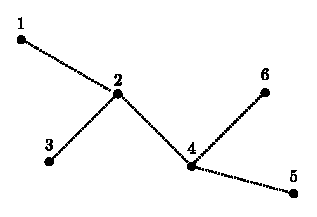
\includegraphics[width=0.55\linewidth]{pic/topology_simple.eps}
	\caption{Example for a tree graph with $N=6$ nodes.}
	\label{fig::topology1}
\end{figure}

Let $(\mathcal{N},\mathcal{E})$ denote a graph with node set $\mathcal{N}=\{1,...,N\}$
and edge set $\mathcal{E}\subseteq \mathcal{N}\times \mathcal{N}$, and $\mathcal N_i = \{ j \in \mathcal N \mid (i,j) \in \mathcal E \}$ denotes
the set of neighbors of vehicel $i$. To reduce duplication, we enumerate tree graph $(\mathcal N, \mathcal E)$ to graph $(\mathcal N, \mathcal E^+)$, with
$$\mathcal E^+ = \{ (i,j) \in \mathcal E \mid i < j \} \; .$$

Refer to ~\cite{JiangTree}, a standard form of tree-structured optimization problems is like following
\begin{equation}
V^* = \min_{x} \; \sum_{ i \in \mathcal{N}} F_{i}(x_i) \quad \text{s.t.} \quad \left\{
\begin{array}{l}
\forall (i,j) \in \mathcal E^+, \\[0.1cm]
S_{i,j}x_{i}=S_{j,i}x_{j}\; .
\end{array}
\right.
\end{equation} 
Here, the functions $F_i: \mathbb R^{n_i} \to \mathbb R$ denote objective functions,
$S_{i,j} \in \mathbb{R}^{n_{i,j}\times n_i}$ and $S_{j,i}\in \mathbb{R}^{n_{i,j}\times n_j}$ given connectivity matrices.

To reformulate the centralized problem, we construct new state variable $$ x_i = (x_i,x_{j,j\in \mathcal{N}_{i}},u_i)$$
and use short hand $d(x_i)\geq\varepsilon$ to collect the collision avoidance constraints ~\eqref{eq::cons4} and ~\eqref{eq::cons3}. Then, the origin problem can be written as following format
\begin{equation}
\label{eq::reform}
V^* = \min_{x} \; \sum_{ i \in \mathcal{N}} J_{i}(x_i) \quad \text{s.t.} \quad \left\{
\begin{array}{l}
\forall (i,j) \in \mathcal E^+, \\[0.1cm]
S_{i,j}x_{i}=S_{j,i}x_{j}, \\[0.1cm]
d(x_i)\geq\varepsilon .
\end{array}
\right.
\end{equation} 



\section{Distributed MPC Scheme}
\label{sec::mpc}
In this section, we propose a distributed MPC scheme outlined in Algorithm~1.
\begin{algorithm}[H]
	\caption{Distributed MPC for Traffic Coordination}	\textbf{Online:}
	\begin{enumerate}
		
		\item \label{MPCstep1} Each vehicle measures $\hat{x}_i$.
		
		\item \label{MPCstep2} Each vehicle communicate with its neighbors to update $a_i$, $\mathcal{V}_i^\mathrm{b}$.

		\item \label{MPCstep3} Each vehicle constructs $x_i$, objective function $J_i(x_i)$, connectivity matrix $S_{i,j}$ and constraint $d(x_i)$.

		\item \label{MPCstep4} Use multi-sweep method to solve~\eqref{eq::reform}.
		
		\item \label{MPCstep5} Each vehicle applies the optimal control $u^*_{i,0}$ during the first one sampling time.	
		
		
	\end{enumerate}
	\label{alg::ALADIN}
\end{algorithm}
Once vehicles receives the new measurement, we need to update the $a_i$ and $\mathcal{V}_i^b$ based on current states $\hat{x}_i$. Besides, if there exists vehicles plugged into the coordination system as a new neighbors, then we expand vehicles set $\mathcal{V}$.
Once $a_i$, $\mathcal{V}_i^b$ and $x_i$ are updated, Problem~\eqref{eq::reform} is solved by a multi-sweep method, a decentralized optimization algorithm over tree topology. Here, we don't elaborate the details about how this method works in a distributed manner, more details can be found in ~\cite{JiangTree}. After that, the first step of optimal solution $u^*_{i,0}$ is applied.

\section{Case Study}
\label{sec::case}
\subsection{Intersection scenario}


\subsection{Lanes merge scenario}


\section{Conclusion}
\label{sec::conc}


\bibliographystyle{plain}
\bibliography{ref}

\end{document}